\documentclass{article}
\usepackage{multicol}
\usepackage{xcolor}
\usepackage[left=1in, right=1in, top=1in, bottom=1in]{geometry}
\usepackage{indentfirst}
\usepackage{graphicx}

\title{Detailed Methods}
\author{DuBose and de Roode}
\date{20XX}

\begin{document}
\maketitle

\begin{multicols}{2}
    \section{Experimental design}
    \indent The objective of this study was to determine how \emph{O. elektroscirrha} infection and plant diet impacts the gene expression of 
    monarchs throughout their development. Infection status (infected and uninfected) and plant diet (\emph{A. incarnata} and \emph{A. curassavica}) 
    were factorially manipulated, resulting in four treatment groups consisting of forty individuals each. The developmental stages 
    sampled in this study were third instar, fifth instar, early pupa (1 day after pupation), late pupa (6-8 days after pupation), and 
    adult (the day of eclosion). Eight caterpillars were sampled at each developmental stage, and from these eight, five were sent for 
    transcriptome sequencing. The overall experimental design is depicted in Figure 1.

    \section{Milkweed cultivation}
    \indent \emph{A. incarnata} and \emph{A. curassavica} seeds were purchased from Joyful Butterfly (Blackstock, SC, USA). To break 
    cold dormancy, seeds were placed in sand-filled bags and kept in a refrigerator at 4°C for two months prior to sowing. Approximately two 
    months before the start of the experiment, seeds were sown into Lambert LM-GPS germination soil and placed in a temperature controlled 
    greenhouse room held between 25°C and 29.4°C. \emph{A. incarnata} germination rates tend to be relatively low, so seed trays were topped with 
    vermiculite to aid in moisture retention. Seedlings were fertilized with approximately X PPM of Jack’s LX 15-5-15 with 4\% Ca and 2\% 
    Mg fertilizer three times a week until the majority of plants grew two sets of true leaves. All plants were then re-potted into Pro-mix 
    BK25 soil, moved to a new temperature controlled room held between 25.6°C and 29.4°C, and fertilized three times a week as described above. 
    Approximately one week before the start of the experiment, plants were moved into the same greenhouse room that caterpillars were reared in 
    (described below).

    \section{Monarch rearing}
    \indent Monarch butterflies were caught and labeled near St. Marks, Florida, U.S.A. (30°09′33″N, 84°12′26″W) between October 21st and 
    October 23rd, 2022. Clear tape was placed on the abdomend of each butterfly and examined under a stereomicroscope to check for 
    \emph{O. elektroscirrha} spores. Prior to mating season, wild-caught monarch butterflies were stored in glassine envelopes, placed in a 
    refrigerator (14°C) to induce a state of diapause, and occasionally fed approximately 10-20\% honey water. Between March 6th and 
    March 15th, 2023, wild-caught monarchs were placed in mesh cages for mating. Each cage was set up in a climate controlled growth chamber 
    (25°C, 16-hour/8-hour day/night cycle) and contained three to six male and three to six female butterflies (Figure 2). All cages were provided 
    with a petri dish containing a sponge soaked in approximately 10-20\% honey water for butterfly feeding. Mating cages were checked every 14 hours, 
    and copulated butterflies were transferred to their own separate cage. After a copulated pair had detached the next day, the male was removed from 
    the cage and the female was given a potted \emph{A. curassavica} plant for oviposition, as well as honey water as described above (Figure 3). After a 
    given female was done laying eggs, the plant was taken out of the growth chamber and placed in a temperature controlled greenhouse room held between 
    23.3°C and 27.8°C for the eggs to hatch. 

    \indent F1 caterpillars were then reared on \emph{A. curassavica} in the same greenhouse room previously described. After pupation, the silk 
    attached to the end of the pupal cremasters was used to hot glue the pupae to the lid of clear solo cups, which were then taken from the 
    greenhouse to the lab (~22°C) for eclosion. A piece of paper towel was placed in the bottom of cups to help absorb liquids produced during 
    the eclosion process. After eclosion, butterflies were placed in glassine envelopes and stored in a refrigerator as previously described. 
    \\
    \\
    \\
    \includegraphics[width=80mm]{../../images/monarch_mating_cages.jpg} \\
    \\
    \includegraphics[width=80mm]{../../images/monarch_feeding_on_honey_water.jpg} \\
    \caption{\textbf{Figure 2.} Top: Monarch butterflies in mating cages. Image does not depict the actual cages used in this experiment.
                                Bottom: Monarch butterfly feeding on honey water from sponge in petri dish.
                                Images do not show actual butterflies used in this experiment.} \\
    \\
    \indent Between April 23rd and May 1st, 2023, F1 butterflies not infected with \emph{O. elektroscirrha} and from different lineages were mated as 
    previously described in the F0 generation. F1 females were given either \emph{A. curassavica} or \emph{A. incarnata} for oviposition, and caterpillars 
    were collectively placed on their treatment plant species upon hatching. Care was taken to make sure caterpillars that had taken bites of 
    the plant they were oviposited on to were placed on the same milkweed species. Likewise, only caterpillars that had not taken any bites of 
    the plant they were oviposited on were placed on the other milkweed species (Figure 1). To reach the sample size needed for this experiment, 
    we used F2 caterpillars from two different lineages that did not share F0 or F1 ancestors. Treatments of parasite infection, plant species, 
    and development stage were randomly distributed to caterpillars from both lineages to minimize confounding due to genetic background.
    \\
    \\
    \\
    \includegraphics[width=80mm]{../../images/monarch_oviposition_cages.jpg} \\
    \\
    \includegraphics[width=80mm]{../../images/monarch_on_oviposition_plant.jpg} \\
    \caption{\textbf{Figure 3.} Top: Female monarch butterflies in cages with \emph{A. curassavica} for oviposition.
                                Bottom: Close-up of female monarch butterfly ovipositing on \emph{A. curassavica}.
                                Images do not show actual butterflies used in this experiment.} \\

    \section{\emph{O. elektroscirrha} inoculation}
    \indent Once caterpillars reached the third instar, parasite treatments were administered. [Details about OE spore acquisition]. 
    \emph{O. elektroscirrha} inoculation was performed by placing caterpillars into petri dishes containing a milkweed leaf disc corresponding to 
    their milkweed treatment group. Prior to placing milkweed leaf discs into the petri dishes, qualitative filter paper was placed into petri 
    dishes and wetted with deionized water to prevent leaf discs from drying out before the caterpillars could finish eating them. Milkweed 
    leaf discs (approximately 6.35 mm in diameter) were obtained by using a standard hole puncher to take sections of the leaf that included 
    side veins but not the midrib, as third instar caterpillars often do not eat leaf midribs. The hole puncher was cleaned using 75\% ethanol 
    between plants to minimize contamination of leaf discs with the other plant species’ chemicals. For infected treatments, 100 \emph{O. elektroscirrha} 
    spores were counted using a stereomicroscope and placed on the veins of the milkweed leaf discs using a modified glass stir rod. Leaf discs fed 
    to uninfected caterpillars were punched at the same time but did not have parasite spores placed onto them. 
    \\
    \indent After all petri dishes and leaf discs were prepared, second instar caterpillars were taken from the plant they were feeding on and placed 
    in a petri dish containing a leaf disc corresponding to their treatment (Figure 4). After caterpillars finished eating their whole leaf discs, they were placed 
    on new plants corresponding to their treatment plant species. Transparent plastic tubes with mesh nets on top were placed around all plants to 
    confine the caterpillars. All tubes were placed on the same shelf in the greenhouse room to minimize possible micro-climate variation, 
    and tube positions were shuffled every three days (Figure 5).
    \\
    \\
    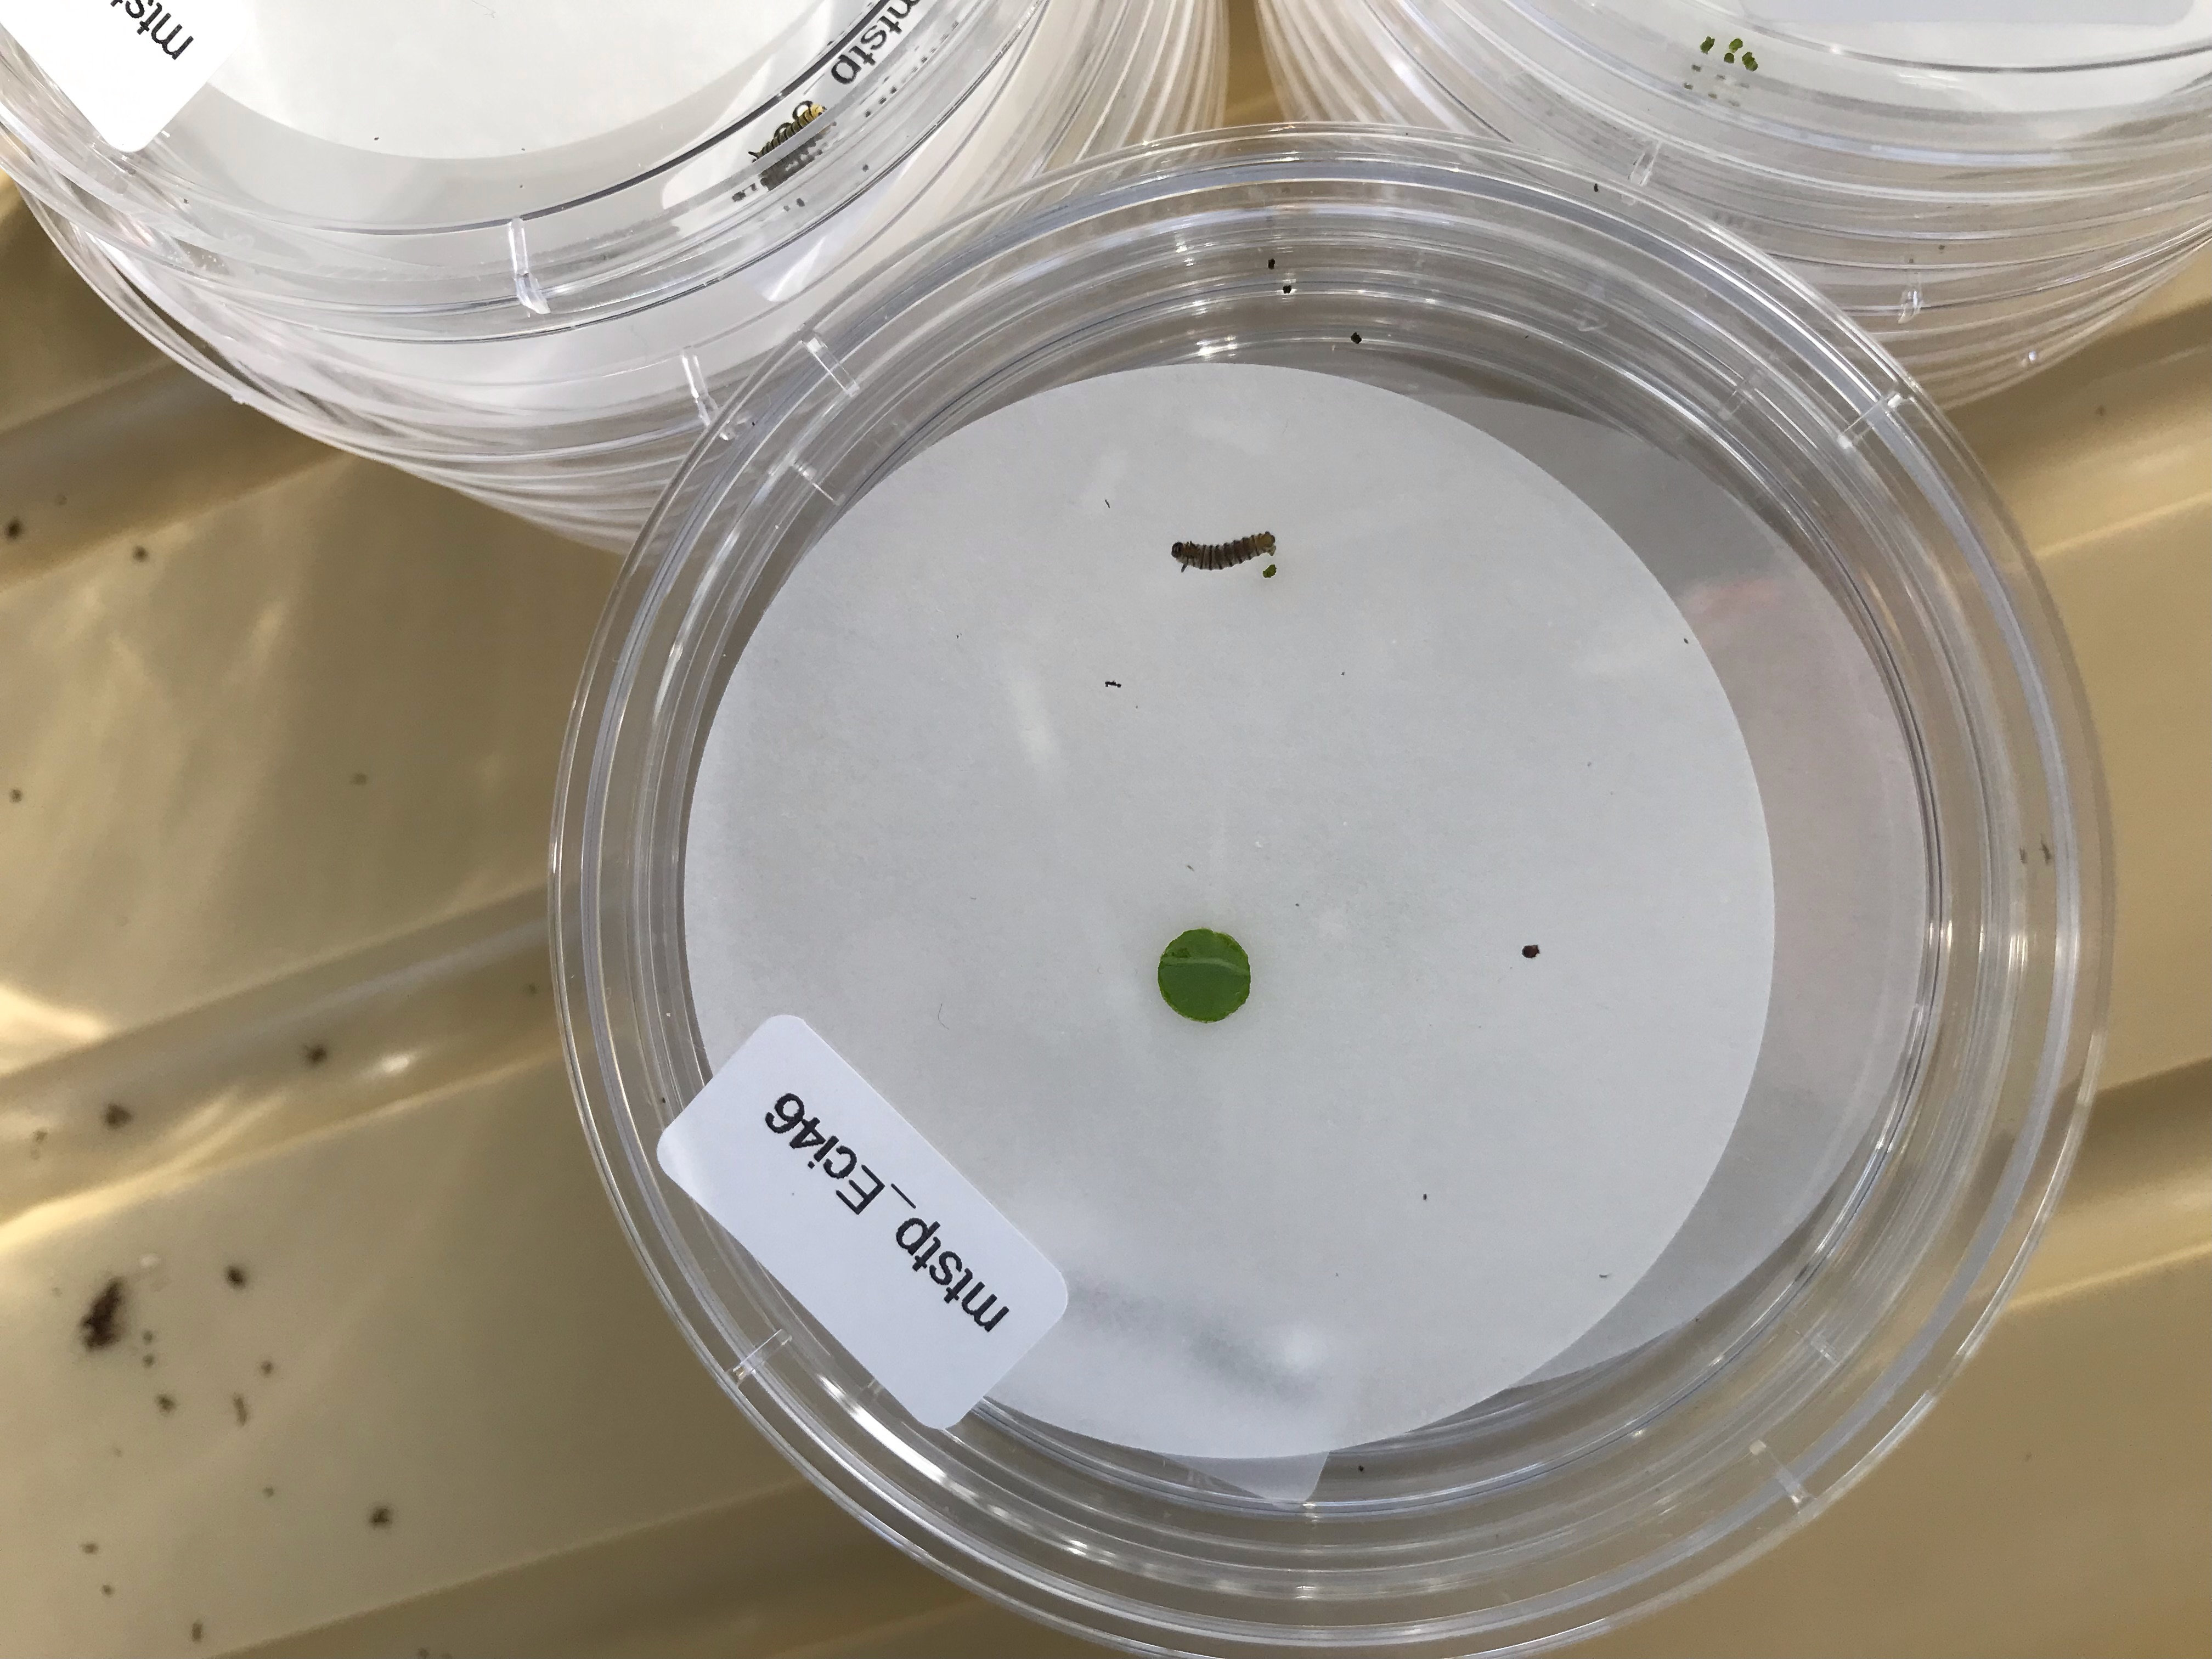
\includegraphics[width=80mm]{../../images/third_instar_in_leaf_disc_dish.jpg} \\
    \caption{\textbf{Figure 4.} Third instar caterpillar in petri dish with milkweed leaf disc.}

    \section{Sampling across developmental stages}
    \indent To minimize changes in transcription due to cold stress, all caterpillars, pupae, and adults were snap frozen in liquid nitrogen before 
    storage in -80°C. Third instar caterpillars were frozen the day after parasite inoculation. Caterpillars were pulled from their feeding plant 
    and quickly placed into a sterile 2mL microcentrifuge tube that was then dipped in liquid nitrogen. Fifth instar caterpillars were frozen in 
    the same way, but were placed in sterile 5mL centrifuge tubes. Caterpillars that ate all of the leaves off of the plant they were originally 
    placed on were placed on another plant of the same species. 
    \\
    \\
    \includegraphics[height=80mm, angle=90]{../../images/greenhouse_exp_tubes.jpg} \\
    \caption{\textbf{Figure 5.} The arrangement of plant tubes on the greenhouse shelf that they were placed on for the duration of the experiment.}\\
    \\
    \indent One day after pupation, early pupa samples were placed in 5mL centrifuge tubes and frozen in liquid nitrogen as described above. 
    Three days after pupation, pupae assigned to late pupa and adult stages were removed from their plant and taped to the lids of clear solo cups 
    using silk attached to the cremaster (Figure 6). This allows for better assessment of the early signs of \emph{O. elektroscirrha} proliferation, as indicated by 
    pupal darkening (Figure 7). In some cases, not enough silk detached with the pupa, and tape was applied directly to the cremaster. Solo cups were then 
    placed on the bottom rack of the same shelf that the caterpillars were reared on, and shade was provided by placing plastic trays above and to 
    the southeast facing side of the shelf to prevent pupae from burning. A piece of paper towel was placed in the bottom of the cups containing 
    adult samples to absorb fluids produced during the pupation process. \emph{O. elektroscirrha}-infected late pupa samples were frozen in liquid nitrogen 
    six to eight days after pupation, depending on when evidence of \emph{O. elektroscirrha} proliferation was presented. To make the distribution of 
    time spent as a pupa even across treatment groups, an uninfected sample that fed on the same plant species and had been a pupa for the same 
    amount of time was also frozen at the same time as each infected sample (Figure 8). Adult samples were frozen on the same day that they eclosed. Here, 
    adults were removed from their solo cup and quickly placed in glassine envelopes, which were then quickly frozen in liquid nitrogen.
    \\
    \\
    \includegraphics[height=80mm, angle=90, trim={10cm 0 15cm 0},clip]{../../images/pupae_cups_holding_tray.jpg} \\
    \caption{\textbf{Figure 6.} Monarch pupae taped to the lids of clear solo cups.}\\
    \\
    \includegraphics[width=80mm, trim={5cm 6cm 5cm 6cm},clip]{../../images/pupal_score_1.jpg} \\
    \\
    \includegraphics[width=80mm, trim={5cm 2cm 5cm 8cm},clip]{../../images/pupal_score_3_vs_uninfected.jpg} \\
    \caption{\textbf{Figure 7.} Top: Monarch pupa showing early signs of \emph{O. elektroscirrha} infection (pupal score=1).
                                Bottom: An uninfected pupa (left) next to an \emph{O. elektroscirrha}-infected pupa (right, pupal score=3)}

    \indent After flash freezing in liquid nitrogen, samples were stored in a styrofoam cooler full of dry ice until all freezing for that day 
    was completed. This process took approximately one hour or less on any given day, so no sample was on dry ice for more than an hour before 
    being transferred to the -80°C freezer. All freezing took place in the same greenhouse room that the caterpillars were reared in, and no 
    caterpillar left said room throughout the duration of the experiment. \\
    \\
    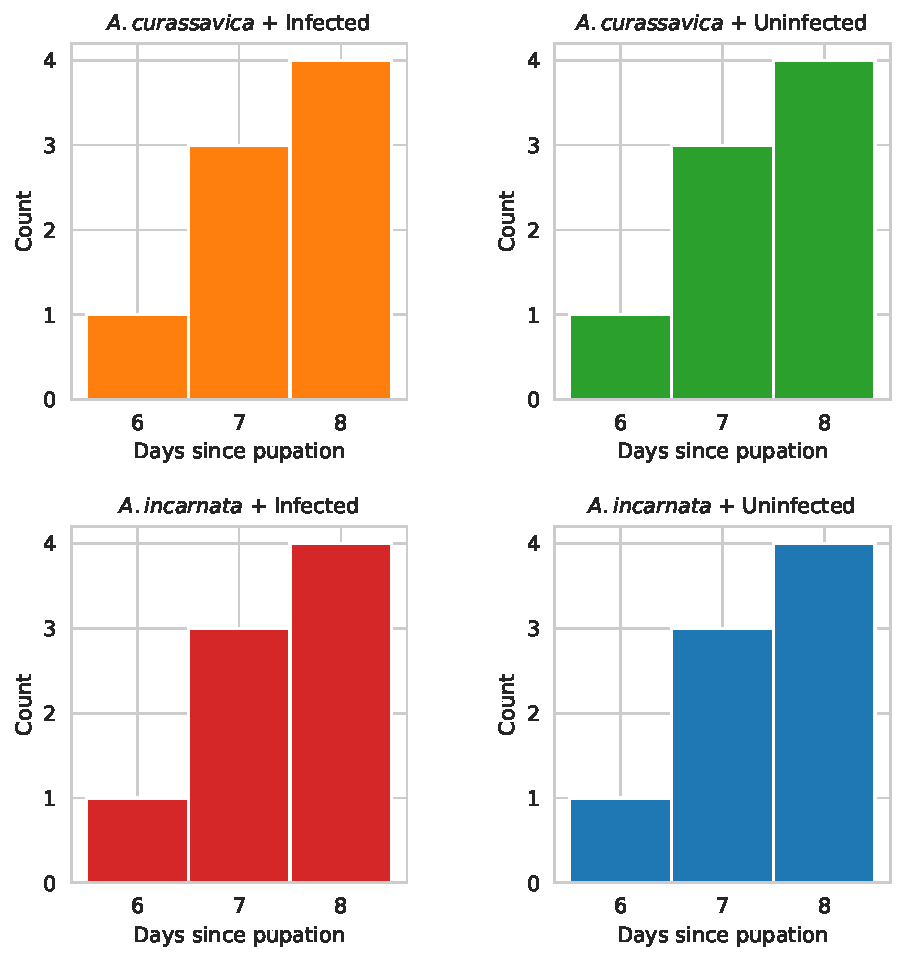
\includegraphics[width=80mm]{../../figures/late_pupal_age_distribution.pdf} \\
    \caption{\textbf{Figure 8.} The distribution of days after pupation that late pupae samples were frozen.}\\
    \\
    \section{RNA Extraction and Sequencing}
    \subsection{\emph{Sample Preparation}}
    \indent 	Prior to RNA extractions, whole caterpillars or butterflies were homogenized by using a porcelain mortar and pestle to grind the tissues into a powder. Mortars and pestles were cleaned using 
    70\% ethanol, and subsequently autoclaved at 121°C while wrapped in aluminum foil. Each sample for a given round of homogenization was removed from the -80°C freezer and placed on dry ice. Samples were 
    individually placed in a sterile mortar and liquid nitrogen was immediately added to prevent samples from thawing. While submerged in liquid nitrogen, samples were ground using a sterile pestle, and liquid 
    nitrogen was continuously added to ensure samples did not thaw throughout the homogenization process. After the sample was completely homogenized, homogenate quickly was collected using a disposable 
    sterile polypropylene spatula (sterilized as described for the mortars and pestles)  and placed in either a 2mL microcentrifuge tube (for 3rd instars) or a 5mL microcentrifuge tube (for all other samples). 
    The microcentrifuge tube was then stored on dry ice while the remaining samples were completed. After all samples were homogenized, they were placed back in the -80°C freezer. Twenty samples were homogenized 
    per round, and each round took approximately two to three hours. 


\end{document}